\documentclass[12pt]{article}

\usepackage{graphicx}
\graphicspath{ {images/} }

\begin{document}
\title{CIS 425 Assignment 3}
\author{Zhexin Jia}
\maketitle

\noindent 1.a. pass-by-value: 2\\
b. pass-by-reference: 4\\
c. pass-by-value-result: 3\\
\vspace{1mm}\\
2. a. 8\\
b. \\
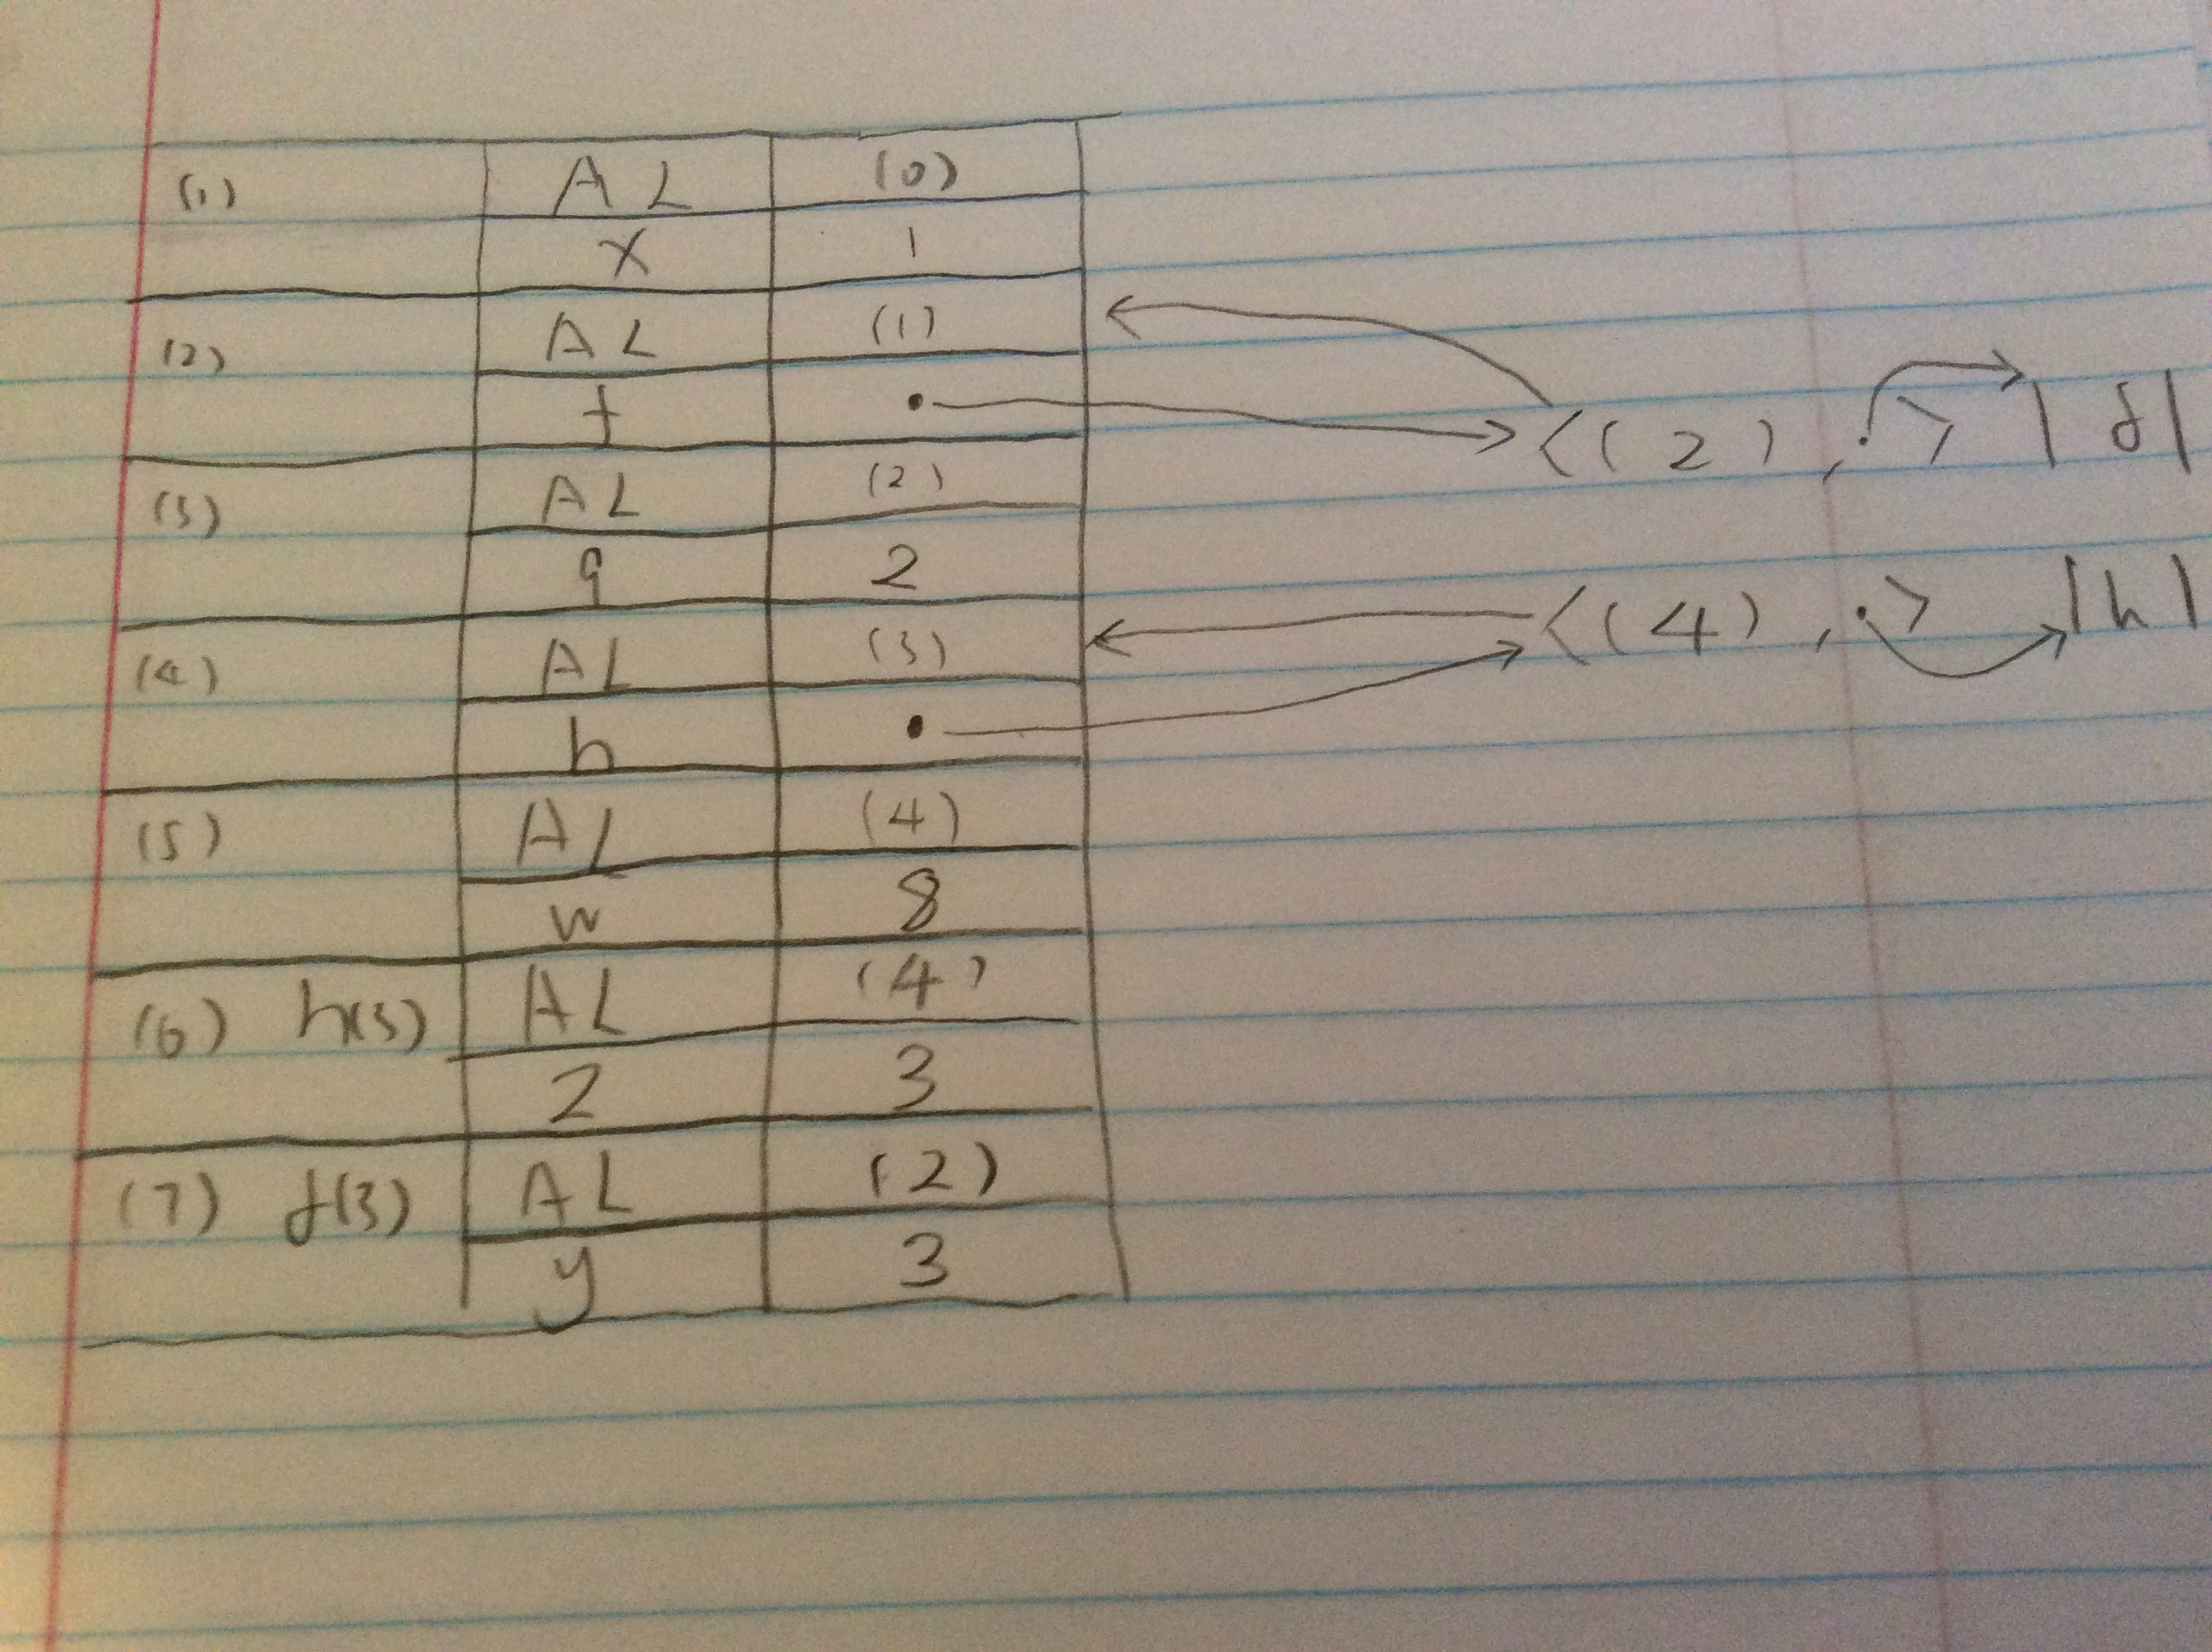
\includegraphics[width=\textwidth]{2b.jpg}
\vspace{1mm}\\
3. (a).\\
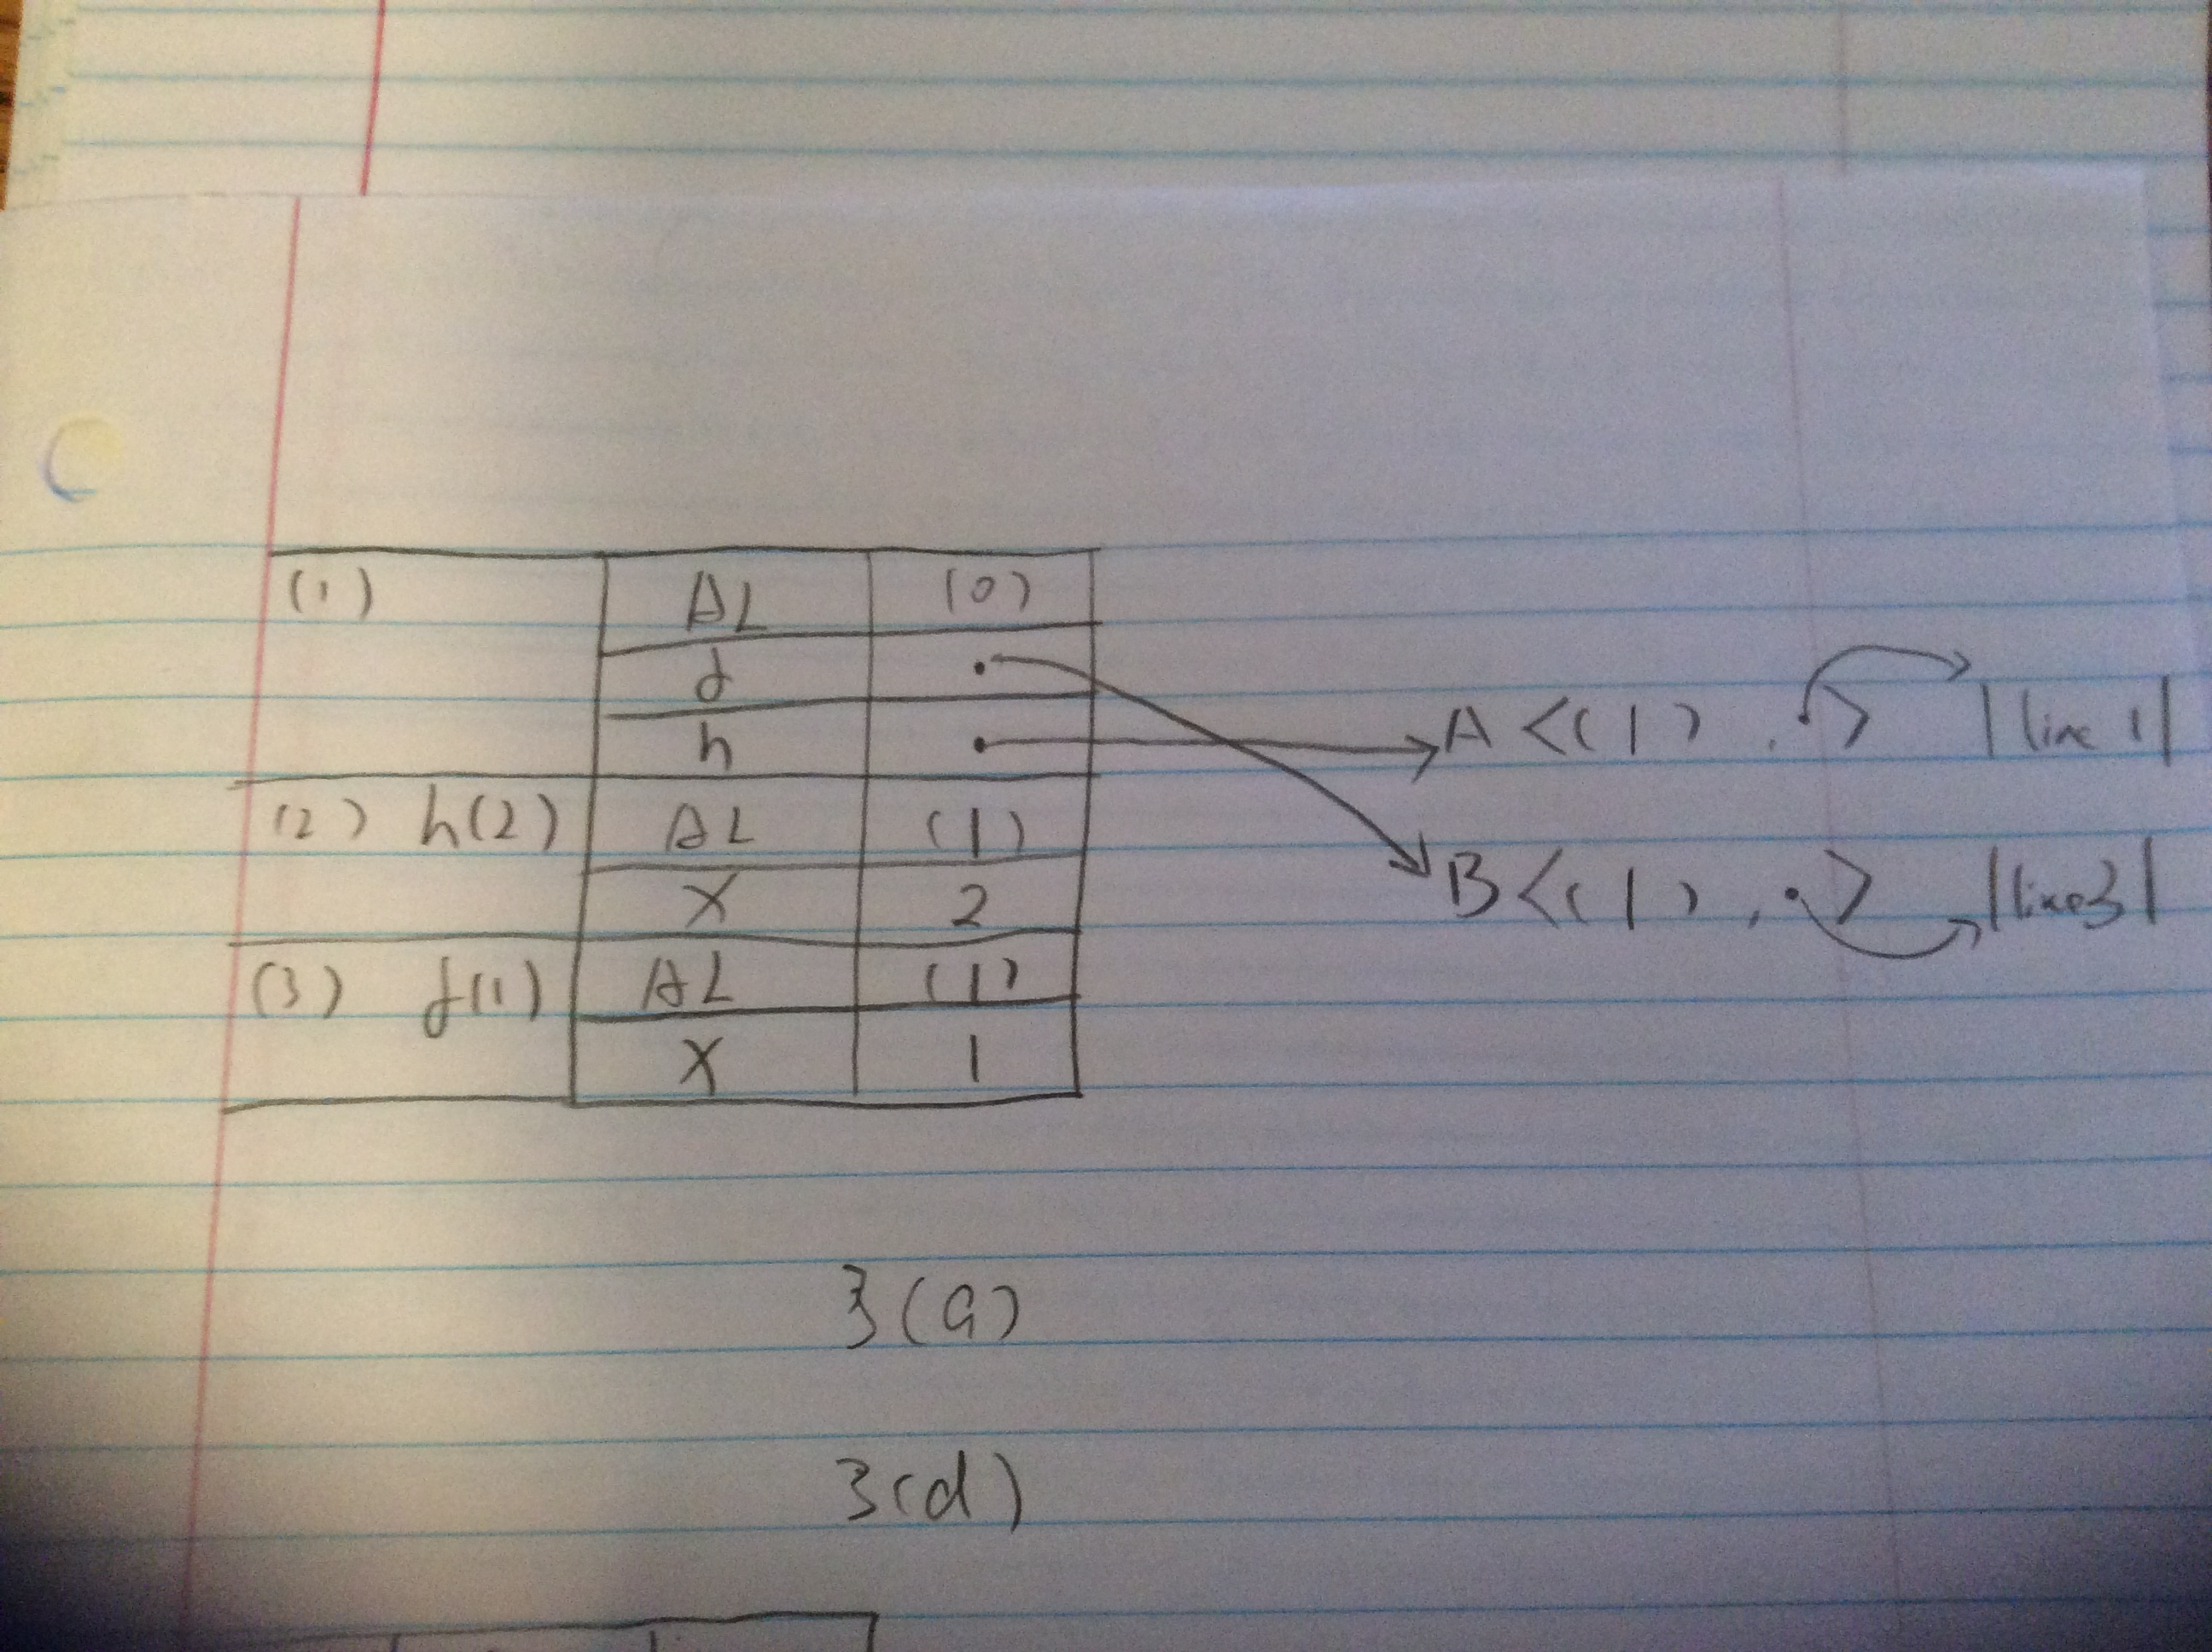
\includegraphics[width=\textwidth]{3a.jpg}
(b). B is used to find the function code for f(1).\\
(c).  We call h(2) after line 2: the function is a recursive function. it keep recursive f1 until x equal to 1. function h and f are both f1. So h(2) return 2*f(2-1), here f is f1, so f(2-1) returns 1, the result is 2*1 = 2.\\
We call h(2) on line 4: the function f has been reassigned to f3, it is not a recursive function any more. h is function f1 and f is function f3. h(2) returns 2f(2-1) = 2*f$_3$(1) = 2*10 = 20.\\
(d). \\
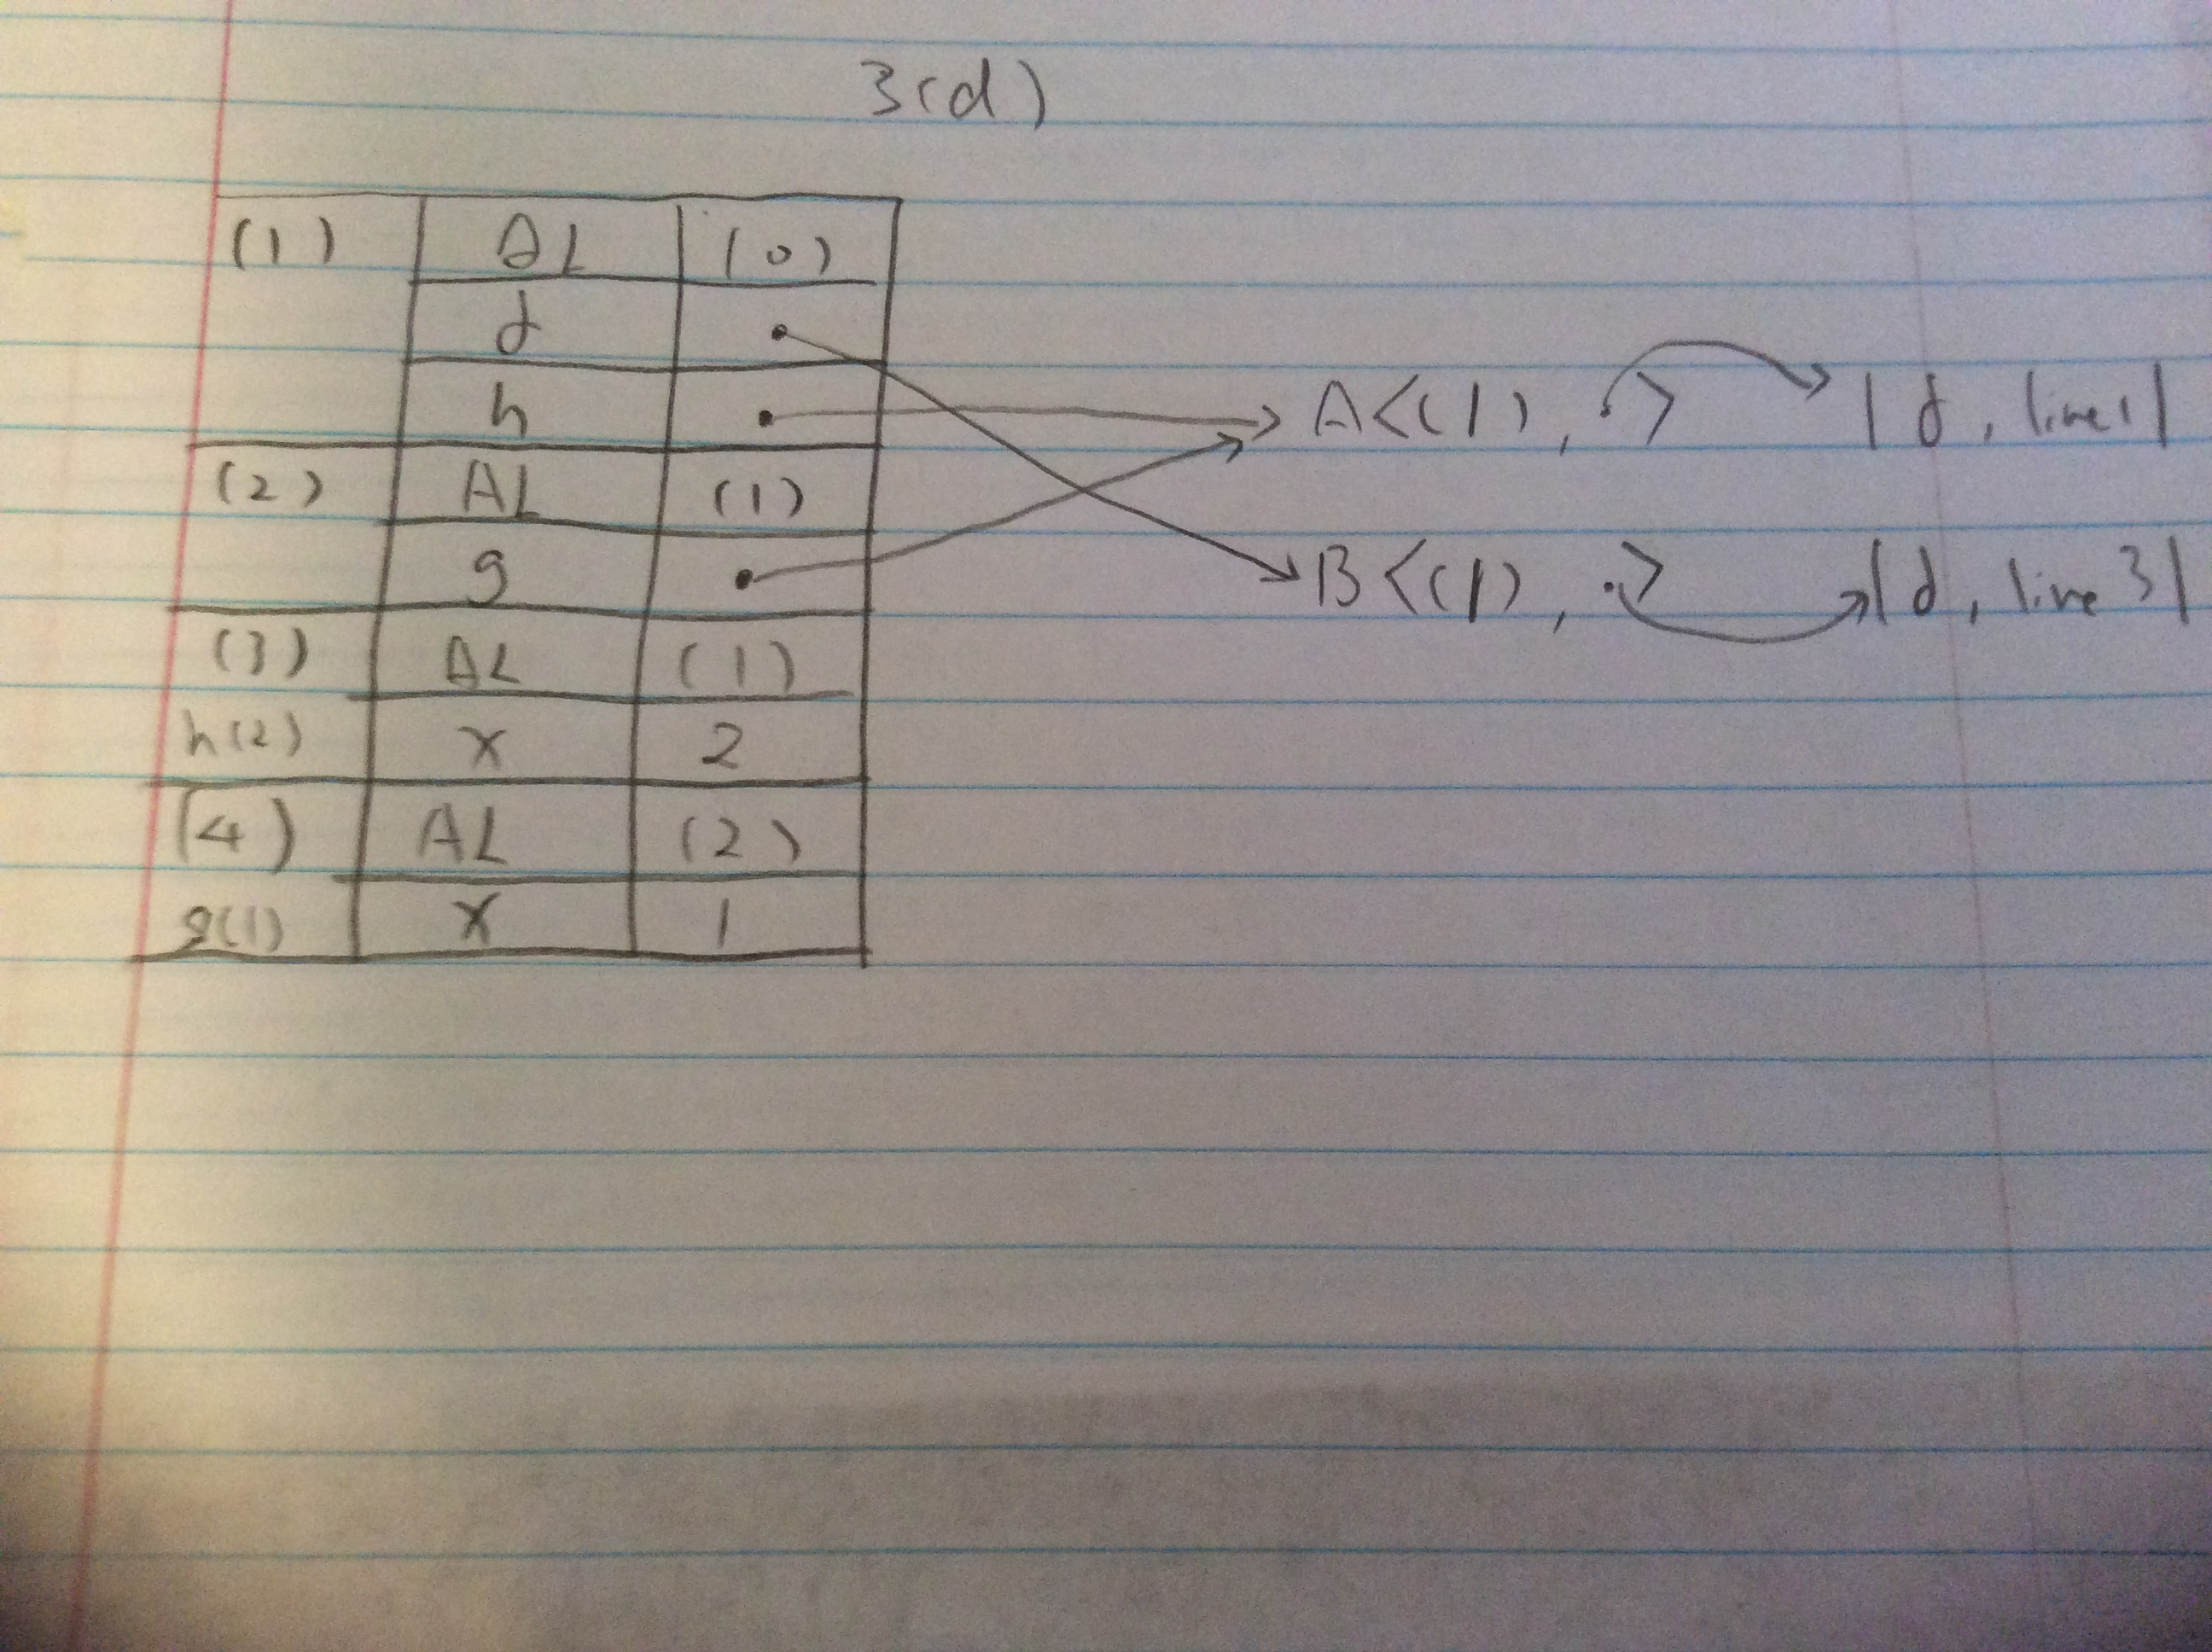
\includegraphics[width=\textwidth]{3d.jpg}
(e). Return 2. Although function f is reassigned to f3, but since we are using a named recursie function, h = f1 keep recurving g(x-1) which is itself, function f is no longer needed. f3 will never be executed no matter which line we call h(2).\\
\vspace{1mm}\\
4. a. 8.\\ 
b. 6.\\
c. There are four x in the function. line 1: foo = function(x)\{...\} is the first x. line 2: ...return function(x) \{return f(f(x));\}... are the second and third x. line 3: ...function(y)\ {return y+x;\}... is the fourth x.\\
The first and fourth x are same, and the second and third x are same. But first and fourth x are not same as the second and third x.\\
The mistake was treating all the x's as the same variable. Correct way is to rename two of them to some other name like 'z'.\\
d. 6\\
\vspace{1mm}\\
5. (a)\\
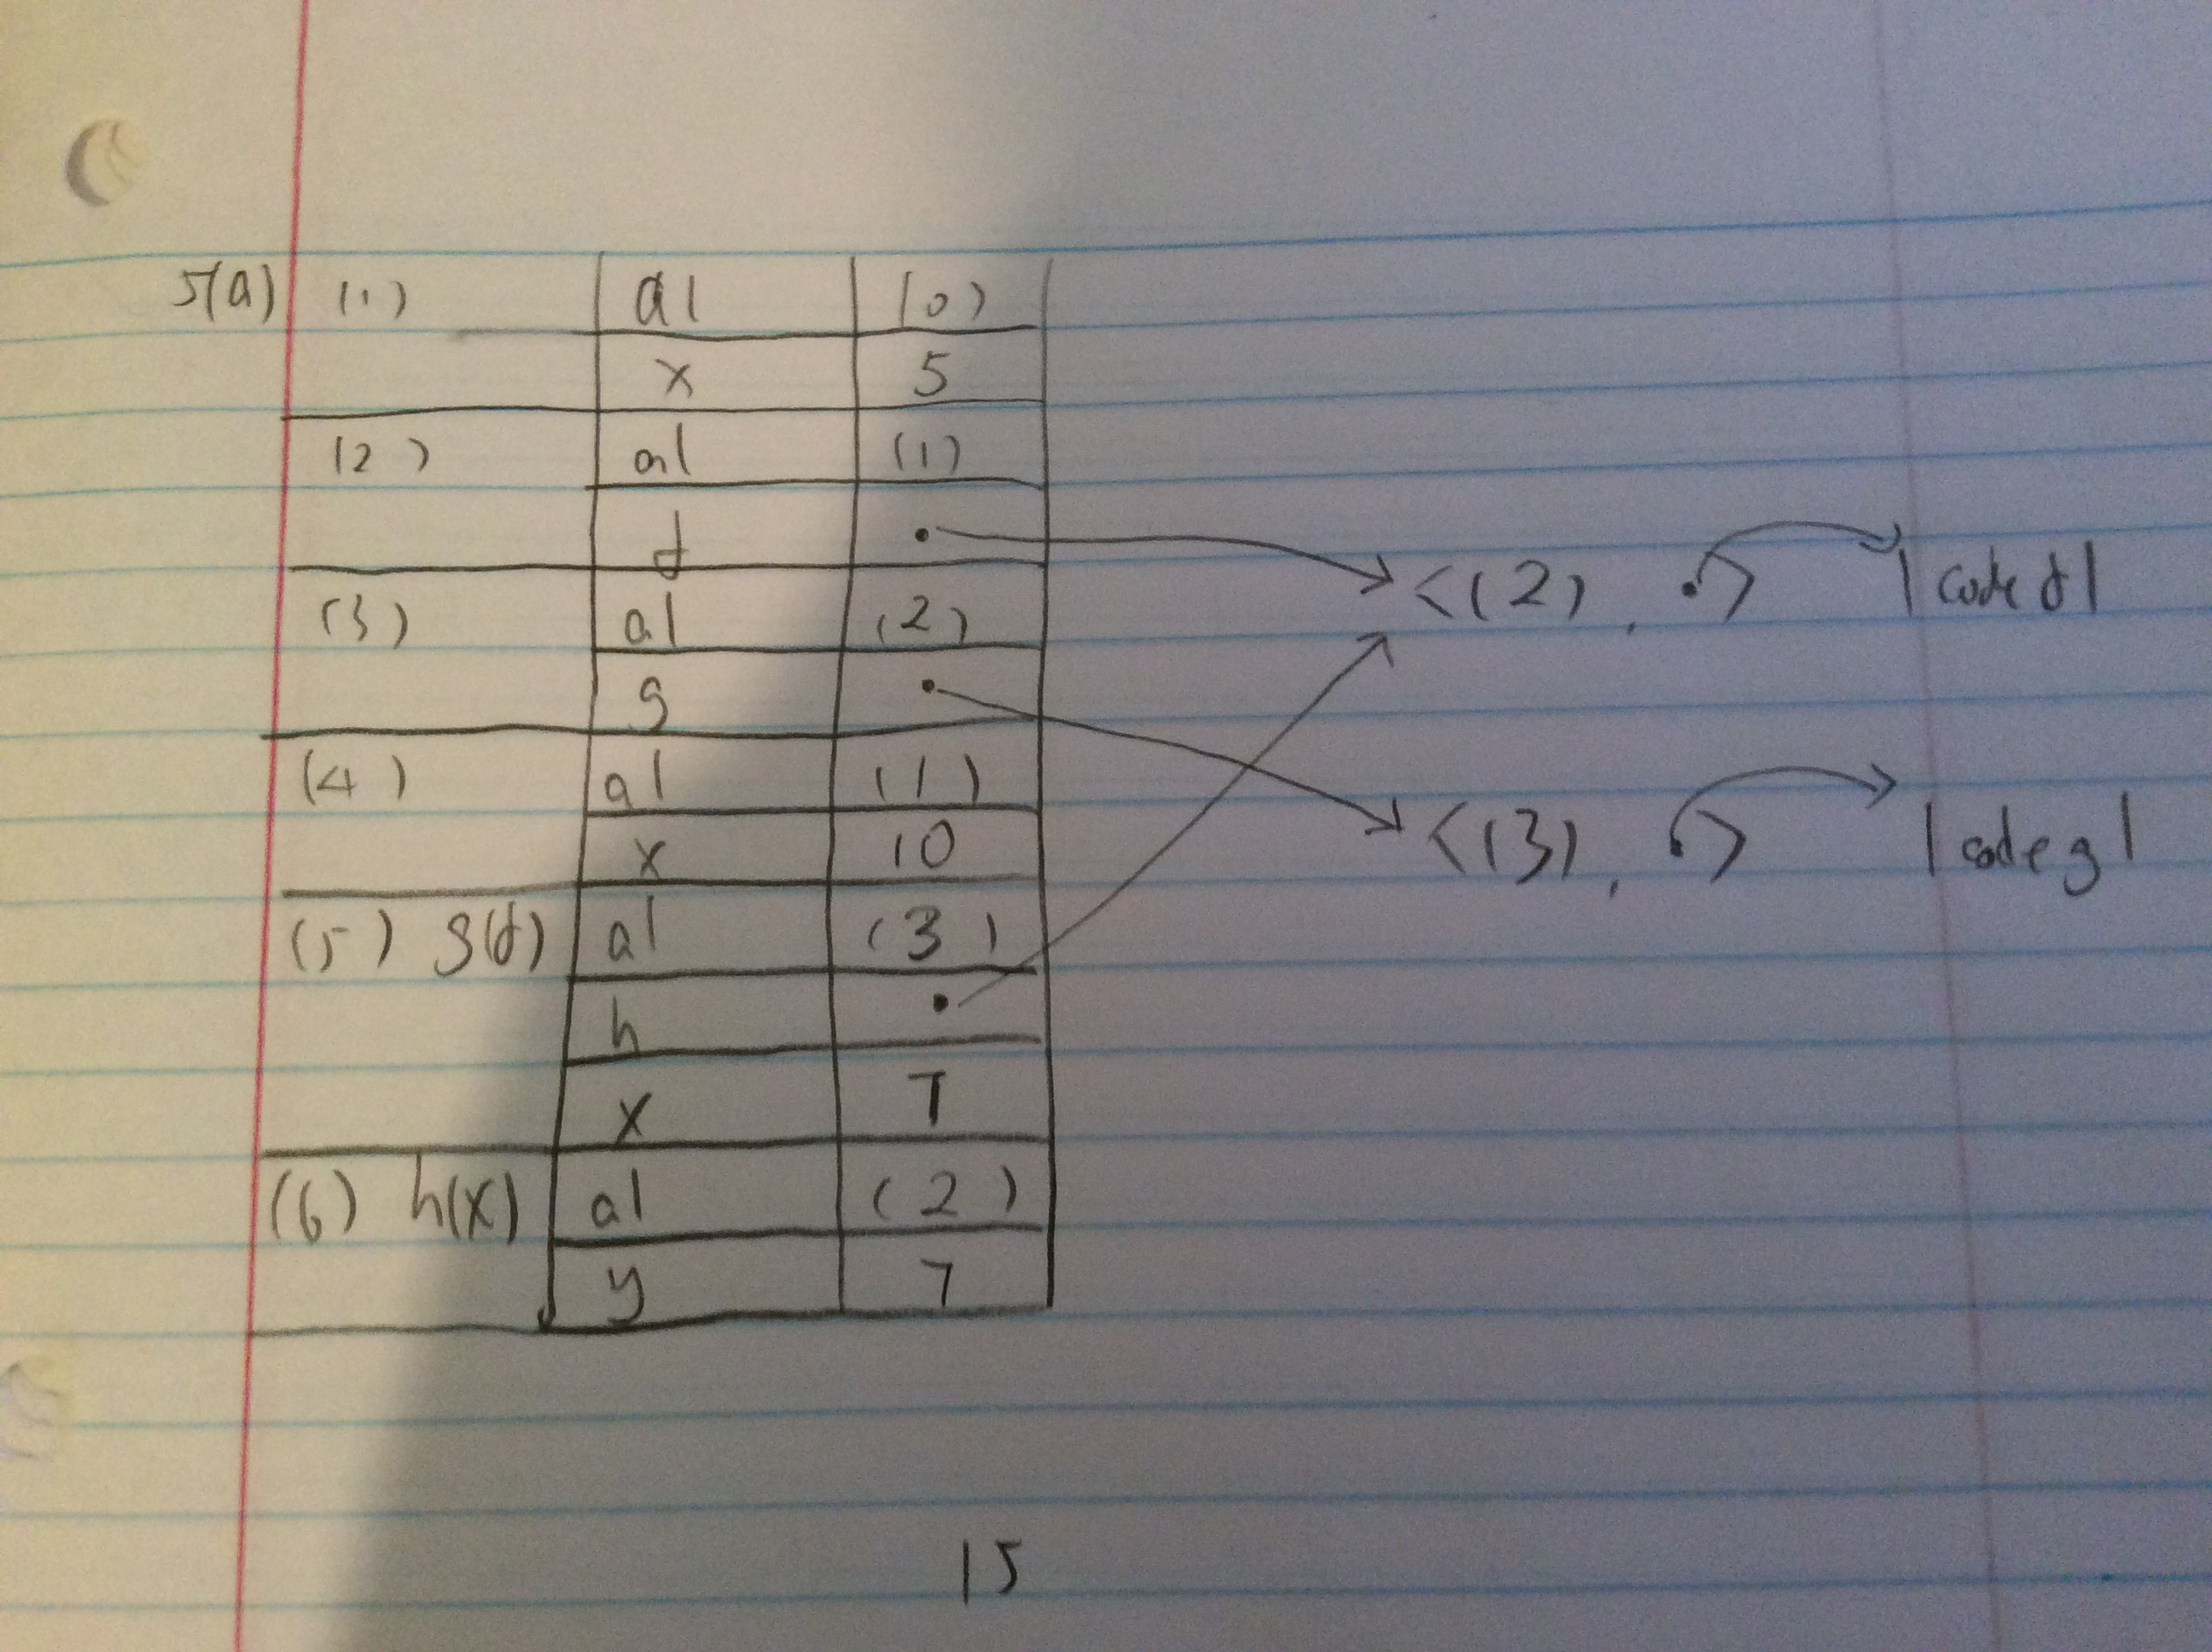
\includegraphics[width=\textwidth]{5a.jpg}
(b). value is 10. x is first assigned to 5, f's access linker link to upper block(x=5 block), it assigns value of x in f to 5.. local x in g is assigned to 7. g(h) return h(x), so after we call g(f), it returns f(7). The paramater of f is the local variable y inside the f. f(y) = f(7), so y is 7. The result is (5+7)-2=10.\\ 
\vspace{1mm}\\
6. (b)\\
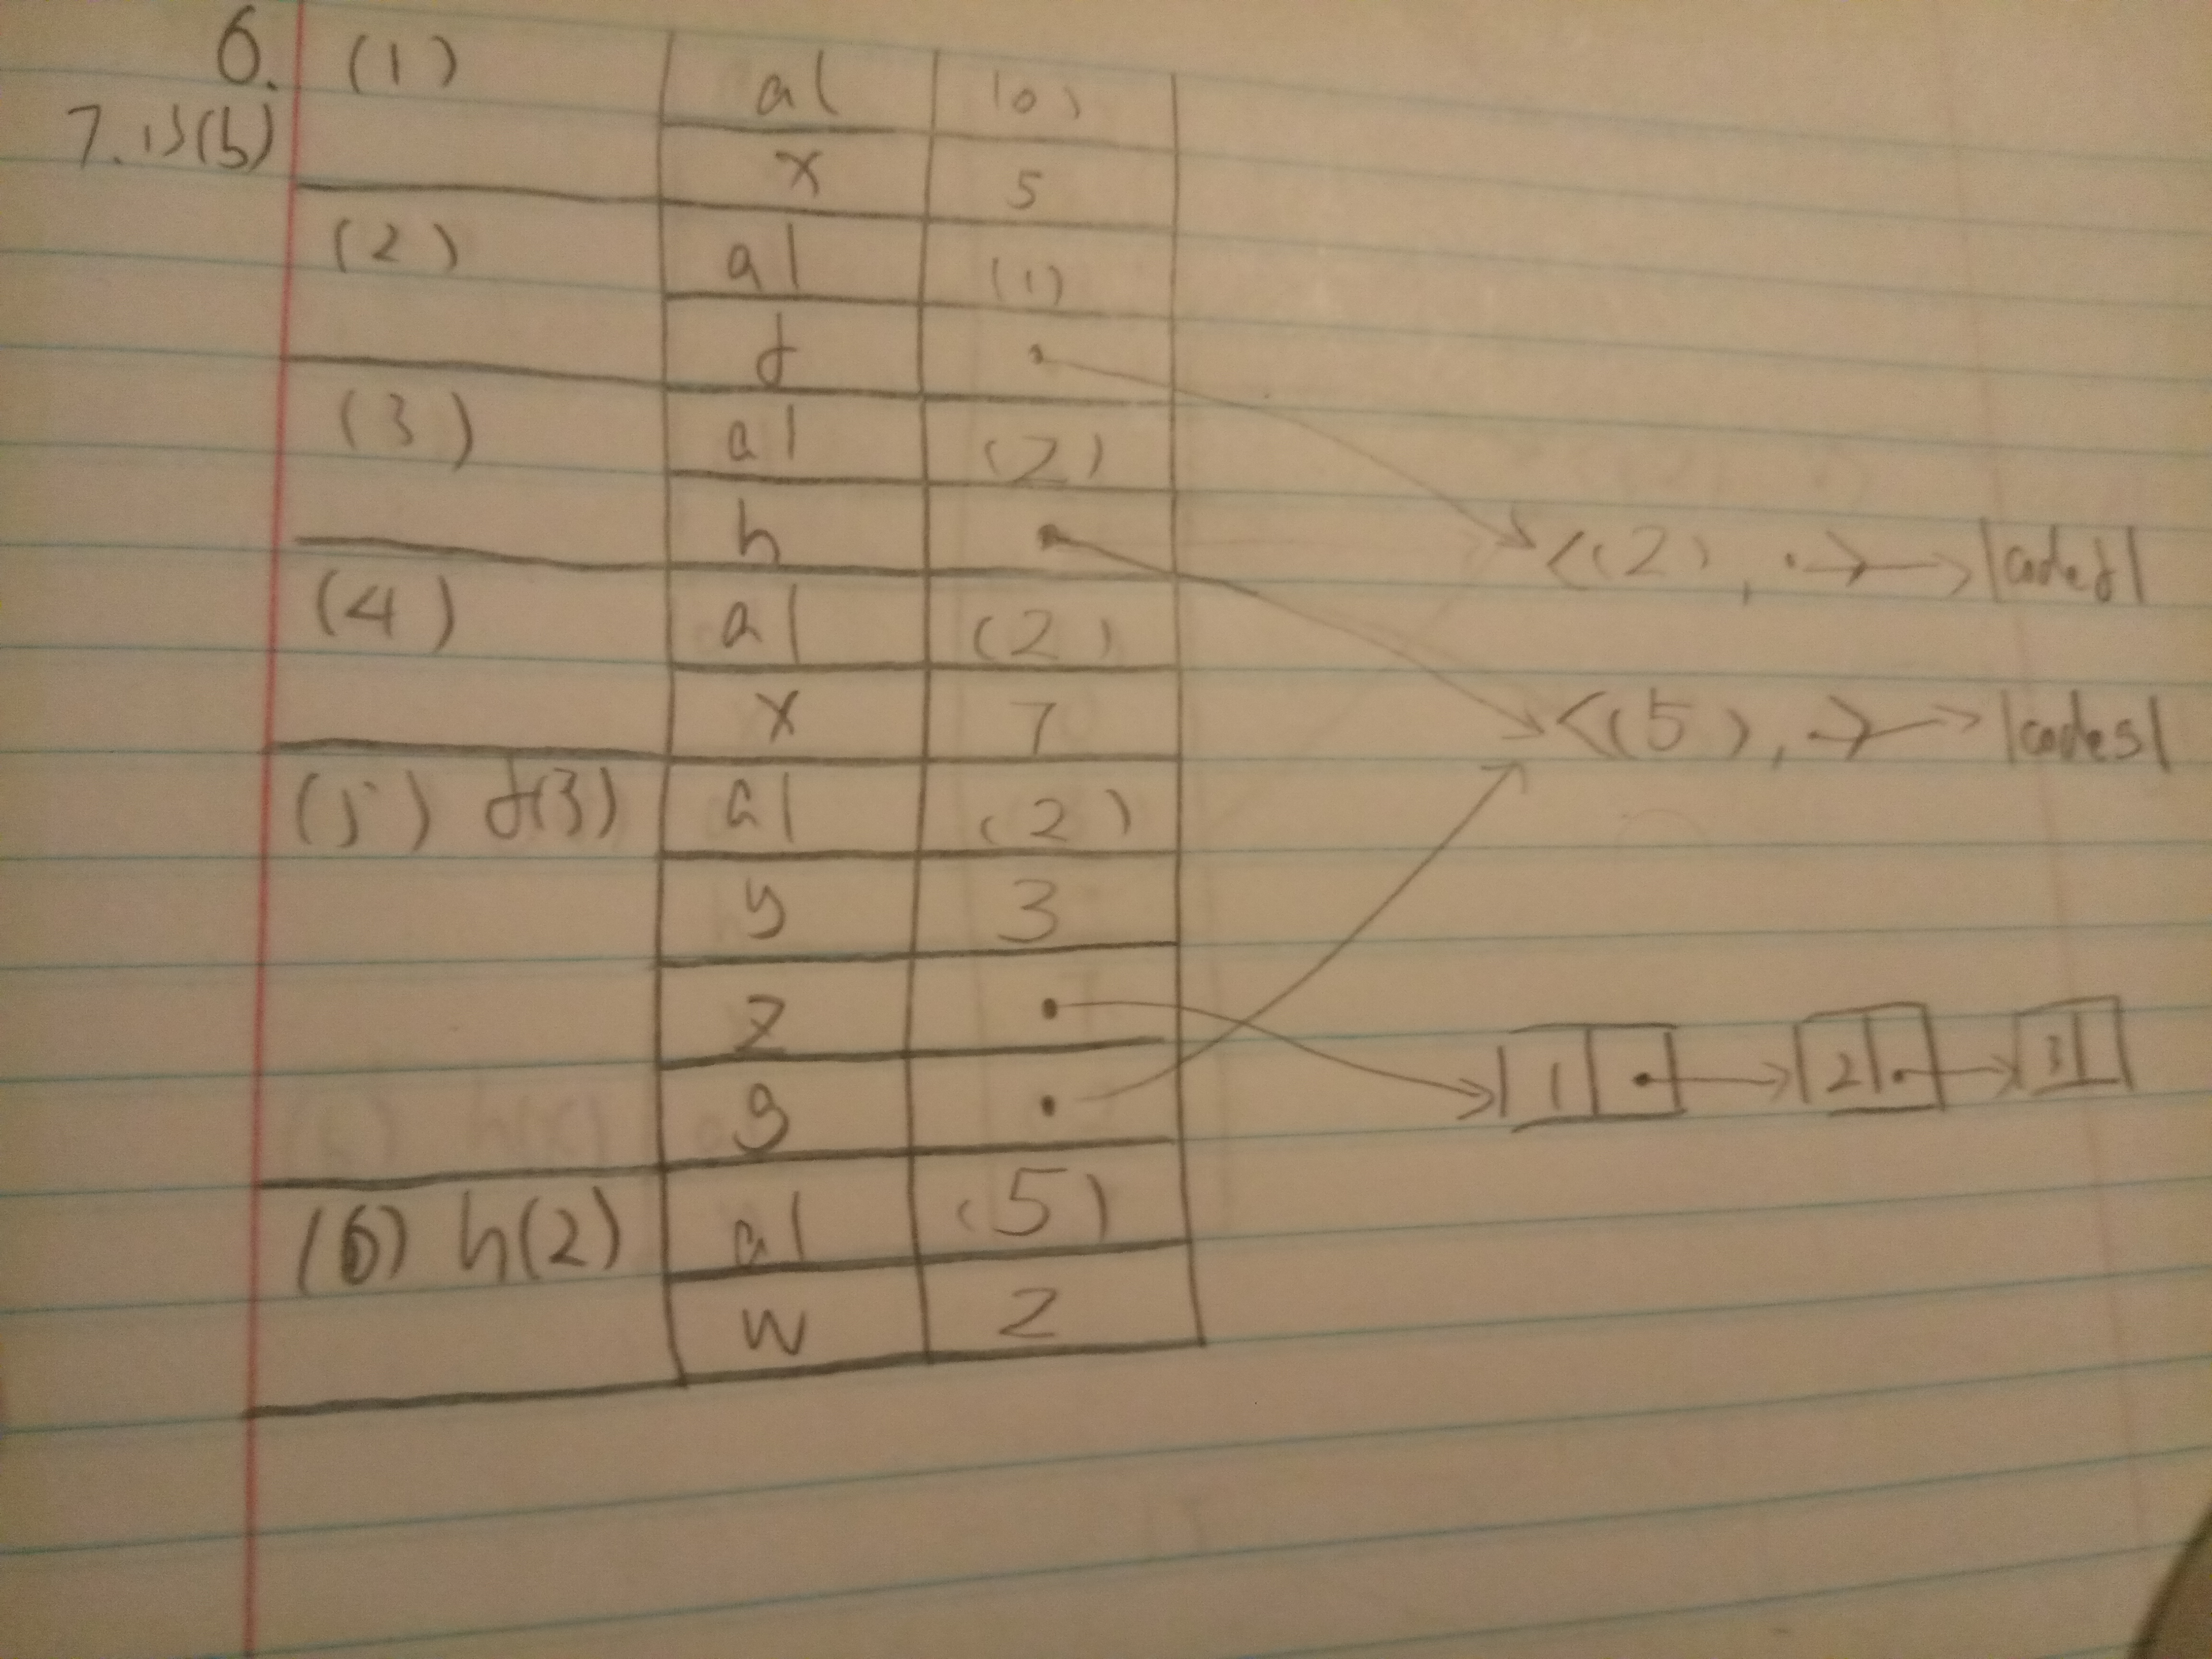
\includegraphics[width=\textwidth]{6b.jpg}
(c). value is 10, w + x + y = 2 + 5 + 3 = 10\\
x = 5 is assigned in the very beginning and never chanced.\\
y = 3 is assigned when function() in h return f(3), y is the parameter of f, so y = 3.
z = 2. h returns f(3), f(3) returns function g, so 2 is setted to be the parameter of g. g(2), w is the parameter of g, so w = 2.
\vspace{1mm}\\
7. ANSI C can not return a function from a function of higher order, closure can pass functions as arguments to other function. so ANSI C can't pass or return a function from a higher order, it does not support closure.\\ 
\end{document}